\chapter{Scrivere documenti scientifici: \LaTeX}
\label{chap:LaTeX}
\mt

\LaTeX\ \`e un programma estremamente potente per la formattazione di
documenti di testo, fortemente orientato alla matematica, che gode di
una notevole popolarit\`a nella comunit\`a scientifica e tra i fisici in
particolare.
In questo capitolo il nostro approccio sar\`a, in un certo senso, minimale:
impareremo come si scrive e compila un documento \LaTeX\ e come si introducono,
all'interno del testo, liste tabelle, equazioni e figure. \`E tutto ci\`o che
verosimilmente pu\`o risultare utile nella redazione di una breve relazione
didattica. Per il resto rimandiamo alla documentazione specifica, che \`e
sconfinata, ed in particolare ai riferimenti bibliografici.


\section{Introduzione}

Prima di entrare nel vivo della discussione, cerchiamo di chiarire alcuni
punti fondamentali che spesso confondono il neofita e che distinguono
\LaTeX\ dai \emph{word processor} pi\`u comunemente usati, come
OpenOffice o Microsoft~Word.

\LaTeX\ \emph{non} fa parte dei programmi di formattazione di tipo \wysiwyg%
\footnote{
Questo orrendo acronimo, che pure si trova piuttosto diffusamente nei manuali
e nella documentazione, sta per l'espressione inglese \emph{What You See Is
What You Get} che, tradotta alla lettera, significa: ci\`o che vedi \`e ci\`o
che ottieni.}%
. L'idea fondamentale che, consapevolmente o meno, sta alla base di questo tipo
di programmi (quelli \emph{a la} Microsoft Word, tanto per intenderci) \`e la
seguente: quello che appare sullo schermo \emph{mentre} scriviamo \`e
sostanzialmente identico al documento finale, come apparir\`a \emph{dopo}
la stampa. Questa idea, che pure sembra cos\`i naturale, tende purtroppo a
nascondere il fatto che la stesura (cio\`e la scrittura vera e propria del
documento, l'organizzazione concettuale del materiale e la scelta delle parole)
e la formattazione (cio\`e la scelta dei caratteri, l'organizzazione della
veste grafica e l'impaginazione) costituiscono due fasi distinte e
concettualmente diverse nella produzione di un documento scritto.
\`E pure evidente che la stesura e la formattazione di un testo richiedono
capacit\`a e competenze diverse e che un ottimo scrittore pu\`o essere un
pessimo tipografo e viceversa.

Facciamo un esempio concreto, tanto per chiarire le idee. Se volessimo dare
inizio ad un nuovo capitolo di un nostro ipotetico documento, quel che la
maggior parte di noi farebbe con un \emph{word processor} di tipo \wysiwyg\
sarebbe con ogni probabilit\`a scrivere il titolo, poi selezionarlo, metterlo
in grassetto, aumentare un po' la dimensione del carattere e magari, a seconda
dei gusti, centrarlo nella pagina. Si tratta di una tipica situazione in cui
si rischia, per cos\`i dire, di \emph{mischiare} il lavoro dello scrittore e
quello del tipografo. Ma vi \`e un'altra cosa importante: nonostante
tutti nostri sforzi e le operazioni di formattazione che abbiamo compiuto,
non vi \`e ancora niente nel nostro titolo che lo qualifichi come tale,
nel senso della struttura del documento, e che lo distingua dal resto del
testo.

In \LaTeX\ l'approccio \`e radicalmente diverso. Un \emph{file} \LaTeX\ \`e
un misto di testo e comandi che sostanzialmente \emph{non} contiene
informazioni riguardanti la formattazione (e dunque, per definizione, non ha
nemmeno la vaga pretesa di apparire simile all'esito finale della stampa).
La formattazione vera e propria avviene invece in un secondo momento, quando
il \emph{file} stesso viene processato con un apposito programma. Tanto per
tornare all'esempio di prima, il titolo del nostro capitolo in un documento
\LaTeX\ verr\`a racchiuso, come vedremo, entro un apposito comando che lo
qualifica effettivamente come titolo di un capitolo e che il programma di
formattazione \`e in grado di riconoscere ed interpretare correttamente a
seconda delle impostazioni definite dall'utente.

Intendiamoci: in alcuni casi (una lettera di poche righe, ad esempio) vi \`e
talmente poco lavoro di tipografia che probabilmente si pu\`o sopravvivere
senza \LaTeX\ (anche se \LaTeX\ ha un bellissimo \emph{template} per le
lettere). D'altra parte anche i programmi di formattazione \wysiwyg, se usati
\emph{propriamente}, consentono di soddisfare la maggior parte delle esigenze.
Ma quando si deve affrontare la redazione di un documento complesso e
voluminoso, \LaTeX\ ha, tra gli altri, l'indubbio vantaggio di
rendere difficile il realizzarlo in modo tipograficamente mal strutturato.
Un motivo sufficiente, quanto meno, per provarlo%
\footnote{
\LaTeX\ \`e un programma \emph{freeware} (cio\`e pu\`o essere scaricato da
web, installato e addirittura redistribuito in modo assolutamente
libero) ed \emph{open source} (cio\`e il codice sorgente \`e aperto,
consultabile e modificabile da tutti).}.


\section{Dalla stesura alla stampa}

Come abbiamo gi\`a detto, un documento \LaTeX\ \`e composto sostanzialmente da
un misto di testo e di comandi \LaTeX\ validi; ne vedremo numerosi esempi
nelle prossime sezioni.
In ogni caso la realizzazione del prodotto finale, pronto per la stampa,
passa attraverso le operazioni fondamentali (cfr. figura \ref{fig:LaTeX})
elencate di seguito:
\panelfig
{\setlength{\unitlength}{\linewidth}
\begin{picture}(1, 0.5)(0, 0)
%\put(0, 0){\framebox(1, 0.5){}}
\put(0.05, 0.25){\framebox(0.1, 0.04){.tex}}
\put(0.15, 0.27){\vector(1, 0){0.1}}
\put(0.25, 0.25){\dashbox{0.004}(0.1, 0.04){\LaTeX}}
\put(0.1, 0.29){\qbezier(0, 0)(0.20, 0.14)(0.40, 0)}
\put(0.2, 0.38){\dashbox{0.008}(0.2, 0.04){Compilazione}}
%\put(0.15, 0.25){\qbezier(0, 0)(0.175, -0.14)(0.35, 0)}
%\put(0.275, 0.13){\makebox(0.1, 0.04){Revisione}}
\put(0.35, 0.27){\vector(1, 0){0.1}}
\put(0.45, 0.25){\framebox(0.1, 0.04){.dvi}}
\put(0.50, 0.29){\qbezier(0, 0)(0.1, 0.25)(0.35, 0.1)}
\put(0.575, 0.46){\dashbox{0.008}(0.2, 0.04){Conversione}}
\put(0.50, 0.25){\qbezier(0, 0)(0.1, -0.25)(0.35, -0.1)}
\put(0.55, 0.27){\vector(3, 4){0.075}}
\put(0.55, 0.27){\vector(3, -4){0.075}}
\put(0.625, 0.15){\dashbox{0.004}(0.1, 0.04){dvips}}
\put(0.625, 0.35){\dashbox{0.004}(0.1, 0.04){dvipdfm}}
\put(0.8, 0.15){\framebox(0.1, 0.04){.ps}}
\put(0.725, 0.37){\vector(1, 0){0.075}}
\put(0.8, 0.35){\framebox(0.1, 0.04){.pdf}}
\put(0.725, 0.17){\vector(1, 0){0.075}}
\put(0.0, 0.){\dashbox{0.008}(0.2, 0.04){Stesura}}
\put(0.1, 0.04){\vector(0, 1){0.21}}
\put(0.5, 0.25){\vector(0, -1){0.21}}
\put(0.40, 0.){\dashbox{0.008}(0.2, 0.04){Visualizzazione}}
\put(0.85, 0.15){\vector(0, -1){0.11}}
\put(0.90, 0.37){\line(1, 0){0.05}}
\put(0.95, 0.37){\vector(0, -1){0.33}}
\put(0.80, 0.){\dashbox{0.008}(0.2, 0.04){Stampa}}
\end{picture}}
{Schema concettuale della preparazione di un documento con \LaTeX.
La prima \`e costituita dalla stesura del documento stesso, che avviene
utilizzando un qualsiasi editor di testo.
Il programma di compilazione permette di creare un'anteprima di come il
documento finale apparir\`a al momento della stampa. In questa prima fase il
documento \LaTeX\ viene tipicamente compilato un numero cospicuo di volte,
fino a che l'autore non \`e soddisfatto del prodotto finale. A questo punto
l'anteprima pu\`o essere convertita nei formati pdf o ps per l'archiviazione,
la condivisione e la stampa.}
{fig:LaTeX}
\begin{numlist}
\item{
Stesura del documento \LaTeX. Qualsiasi editor di testo%
\footnote{
Possiamo citare emacs sotto \linux\ e notepad (blocco note) sotto \windows.
\`E importante notare che i word processor pi\`u avanzati non sono editor di
testo e non servono quindi allo scopo (provare per credere!).
}
va bene allo scopo, ovviamente, anche se vale la pena di notare che alcuni
(sia sotto \linux\ che sotto \windows) possiedono funzionalit\`a specifiche
molto utili%
\footnote{
Tra questi ricordiamo Kile sotto \linux\ e TeXniCenter sotto \windows.
}%
.
Per fissare le idee, se vogliamo creare un nuovo \emph{file} \LaTeX\ chiamato
\cchar{Relazione.tex} usando emacs sotto \linux, digiteremo nella \emph{shell}:
\begin{verbatim}
>emacs Relazione.tex &
\end{verbatim}
}
\item{
Compilazione. Si esegue dal terminale%
\footnote{
Per terminale intendiamo qui sia la \emph{shell} di \linux\ che il
\emph{prompt} di \dos\ nel caso in cui si lavori sotto \windows. Notiamo anche
esplicitamente che, nel caso in cui si utilizzino editor orientati a \LaTeX\
come quelli citati prima, vi sono in generale appositi pulsanti nelle
rispettive interfacce grafiche per l'utente che permettono di eseguire questa
operazione automaticamente.
}
attraverso il comando \ccmd{latex}. Ad esempio per compilare il \emph{file}
\cchar{Relazione.tex} digiteremo:
\begin{verbatim}
>latex Relazione.tex
\end{verbatim}
In questo modo, a meno che non vi siano errori di sintassi all'interno del
documento \LaTeX\ (nel qual caso il compilatore si lamenter\`a e potrete
tornare al terminale premendo \ckey{CTRL + C}), verr\`a prodotto un certo
numero di \emph{file} con diverse estensioni (dvi, log, aux).
Il pi\`u importante \`e senza dubbio il \emph{file} con estensione dvi%
\footnote{
L'estensione .dvi \`e l'acronimo dell'espressione inglese \emph{DeVice
Independent} che, tradotta letteralmente, significa: indipendente dal
dispositivo.
}
che, come vedremo tra un attimo, rappresenta una sorta di \emph{anteprima di
stampa}.
}
\item{
Visualizzazione dell'anteprima. \`E necessario utilizzare un programma in
grado di leggere correttamente il \emph{file} dvi. Sotto \linux%
\footnote{
Sotto \windows\ si usa tipicamente un programma che si chiama yap e che viene
installato automaticamente al momento dell'installazione di \LaTeX.
Se si usano editor di testo con funzionalit\`a specifiche, essi includono
spesso dei bottoni per compiere l'operazione automaticamente.
}
si utilizza tipicamente il comando \ccmd{xdvi}:
\begin{verbatim}
>xdvi Relazione.dvi &
\end{verbatim}
}
\item{
Conversione in un formato adatto per la stampa. Quando siamo soddisfatti del
nostro documento, come appare nel formato dvi, possiamo convertirlo in un
formato adatto per essere archiviato, condiviso o stampato. Tipicamente questo
formato pu\`o essere il postscript:
\begin{verbatim}
>dvips Relazione.dvi -o Relazione.ps
\end{verbatim}
oppure il pdf:
\begin{verbatim}
>dvipdfm Relazione.dvi Relazione.pdf
\end{verbatim}
Nel primo caso creiamo il \emph{file} postscript \cchar{Relazione.ps}, nel
secondo il \emph{file} pdf \cchar{Relazione.pdf}, che possono essere
visualizzati con GhostView ed Acrobat Reader, rispettivamente, oltre che
essere stampati con il comando usuale.
}
\end{numlist}


\section{Il primo documento \LaTeX}
\label{sec:Documento1}

Tanto abbiamo detto sulla compilazione e la stampa che probabilmente \`e
giunto il momento di cercare di capire come effettivamente questo documento
\LaTeX\ vada scritto.

Cominciamo dunque con il pi\`u semplice documento che si possa immaginare
e scriviamo un \emph{file} di testo contente le $4$ linee seguenti:
\begin{verbatim}
\documentclass[11pt, a4paper]{article}
\begin{document}
Il mio primo documento\ldots
\end{document}
\end{verbatim}
Il risultato della compilazione, essenzialmente pronto per essere stampato,
\`e mostrato in figura~\ref{fig:Documento1}.
\panelfig
{\framebox{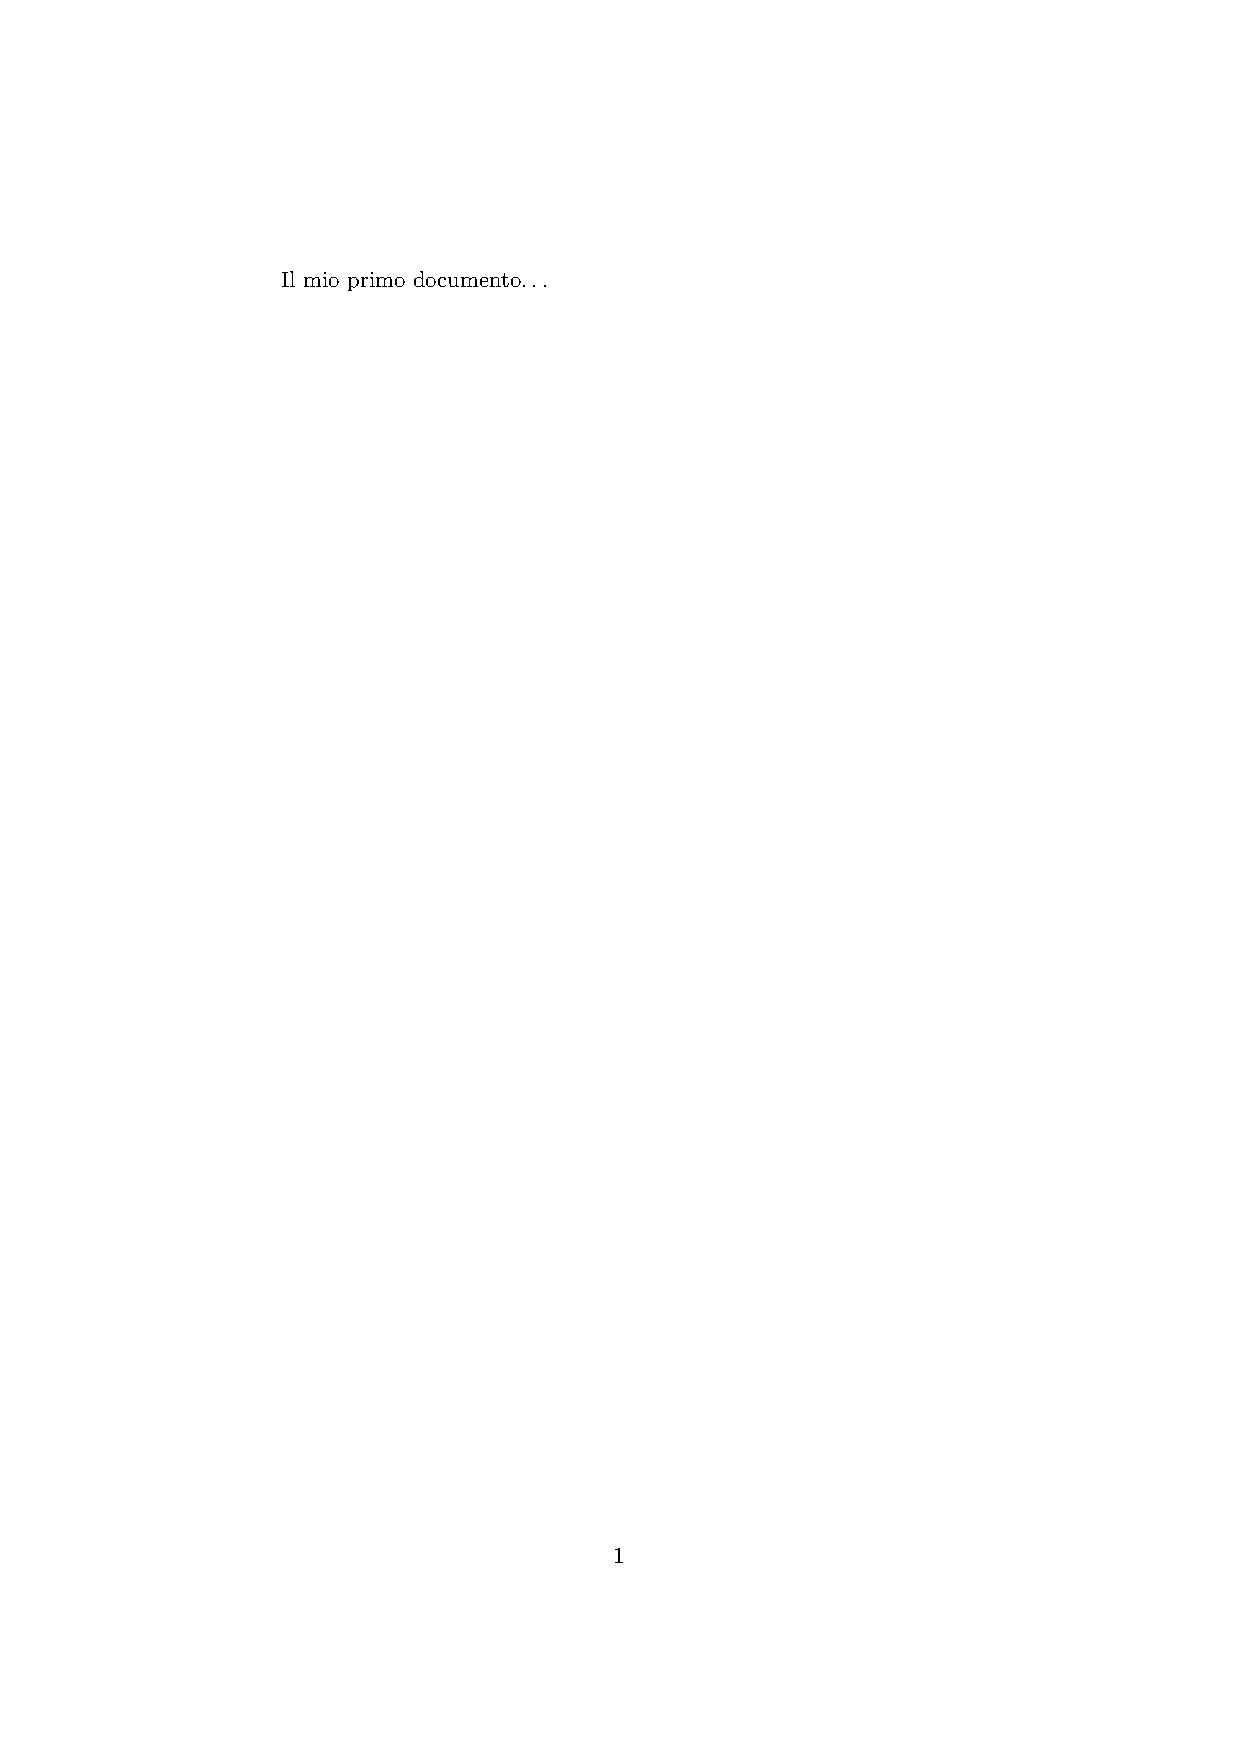
\includegraphics[width=14cm]{./ps_LaTeX/figure/documento1}}}
{Risultato della compilazione del documento \LaTeX\ riportato nel
paragrafo \ref{sec:Documento1}.}
{fig:Documento1}
Non \`e niente di esaltante, bisogna ammetterlo\ldots Ma prima di andare
avanti e familiarizzare con funzionalit\`a pi\`u potenti ed avanzate,
cerchiamo di capire il significato di ciascuna delle quattro righe del nostro
documento. Una per una.

\begin{verbatim}
\documentclass[11pt, a4paper]{article}
\end{verbatim}
Qui dichiariamo sostanzialmente il tipo di documento. Diciamo che si tratta di
un documento del tipo \emph{article}%
\footnote{
Esistono moltissimi tipi diversi di documenti predefiniti in \LaTeX\, tra cui
\emph{book}, \emph{report}, \emph{letter} e \emph{slides}; altri possono essere
aggiunti, anche se non si tratta esattamente della cosa pi\`u semplice del
mondo. Il tipo \emph{article} si presta piuttosto bene alla stesura di una
relazione di media lunghezza su una esperienza didattica ed \`e questo il
motivo per cui lo abbiamo scelto per i nostri esempi. 
}%
, che la dimensione dei caratteri del testo ordinario \`e $11$ punti%
\footnote{
Esistono anche le varianti 10 e 12 punti.
}%
, e che la dimensione della pagina \`e quella di un foglio A4%
\footnote{
Altri formati validi, solo per citarne un paio, sono \emph{a5paper}
e \emph{letterpaper}.
}
(che \`e la scelta tipica).

\begin{verbatim}
\begin{document}
\end{verbatim}
Segna l'inizio del documento vero e proprio. In generale questo comando separa
quello che \`e chiamato \emph{preambolo} (nel nostro caso \`e sostanzialmente
la linea precedente) dal \emph{corpo} vero e proprio del documento, che \`e
\emph{sempre} contenuto tra un comando di inizio ed un comando di fine
documento.

\begin{verbatim}
Il mio primo documento\ldots
\end{verbatim}
Si tratta del corpo del nostro documento, ed in effetti \`e la parte che
compare nella versione pronta per la stampa, come si pu\`o vedere in figura
\ref{fig:Documento1}.

\begin{verbatim}
\end{document}
\end{verbatim}
Questa linea chiude il documento ed \`e sempre richiesta alla fine di un
\emph{file} \LaTeX\ valido.

Nel prossimo paragrafo vedremo un esempio di documento pi\`u realistico e
cominceremo ad apprezzare alcune funzionalit\`a pi\`u utili ed avanzate.


\section{Un documento realistico}
\label{sec:Documento2}

Consideriamo attentamente il documento \LaTeX\ (valido) che segue\ldots

\begin{verbatim}
\documentclass[11pt, a4paper]{article}
\title{Il mio primo documento}
\author{Luca Baldini}
\date{20 Giugno 2006}

\begin{document}
\maketitle

\section{Introduzione}
Questo vuole essere un esempio di documento realistico, con lo scopo
di mostrare alcune tra le funzionali\`a di base di \LaTeX.

\section{Un nuovo capitolo}
Una prima cosa da notare \`e che, una volta dichiarate le sezioni del
documento, \LaTeX\ si occupa automaticamente della numerazione. Questo
pu\`o risultare estremamente utile nel caso in cui si voglia aggiungere
una nuova sezione in mezzo ad un documento in stato avanzato di stesura
(non \`e necessario rinumerare ci\`o che viene dopo, \LaTeX\ fa
tutto da solo). 

\subsection{Una sotto-sezione}
Come vedete esiste anche un livello pi\`u \emph{basso} di sezionamento
del documento.

\subsection{Ancora una sottosezione}
Anche a questo livello la numerazione \`e automatica. Questo consente
anche, in documenti pi\`u complessi, la generazione automatica dell'indice.

\section{Conclusioni}
Per il momento ci fermiamo qui, abbiamo abbastanza di cui discutere\ldots

\end{document}
\end{verbatim}

\noindent \ldots e vediamo come appare l'uscita del compilatore, pronta per
la stampa, che \`e riportata in figura \ref{fig:Documento2}.
\panelfig
{\framebox{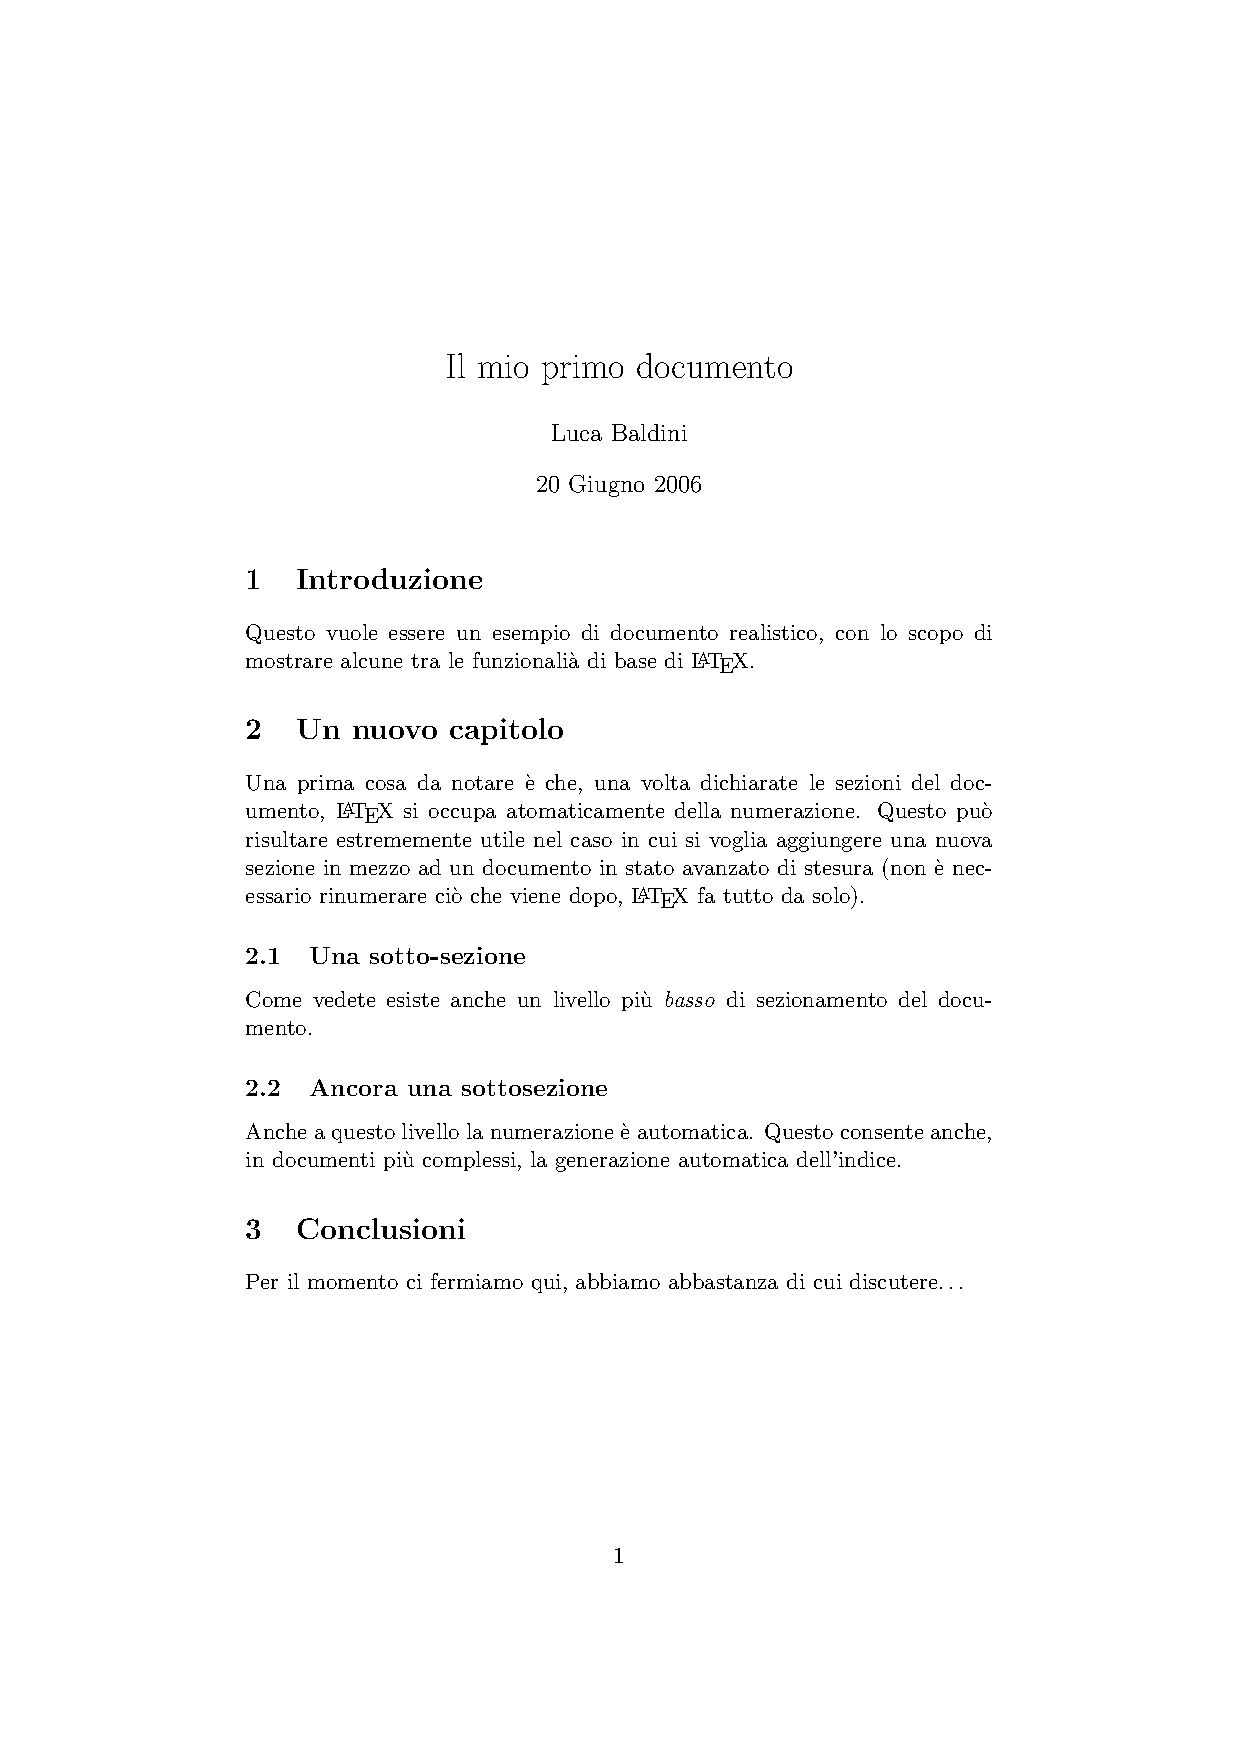
\includegraphics[width=14cm]{./ps_LaTeX/figure/documento2}}}
{Risultato della compilazione del documento \LaTeX\ riportato nel
paragrafo \ref{sec:Documento2}.}
{fig:Documento2}
Cominciamo con alcuni commenti di carattere generale per poi passare
all'analisi di alcuni tra i nuovi comandi che abbiamo appena incontrato.

Tutti i comandi \LaTeX\ cominciano con il carattere ``\verb|\|''
(\emph{backslash}). Alcuni di essi accettano (o richiedono, a seconda del
caso) \emph{opzioni} (che sono sempre contenute tra parentesi quadre) e
\emph{argomenti} (racchiusi tra parentesi graffe).
I comandi ed il testo sono, come \`e evidente, mischiati insieme all'interno
del documento. \`E importante notare come gli spazi multipli siano trattati
come  spazi singoli e come i ritorni a capo siano semplicemente ignorati,
se non che una linea vuota segna l'inizio di un nuovo paragrafo.
Esiste ovviamente un comando per andare a capo ed \`e ``\verb|\\|''
(doppio \emph{backslash}).

Tra i comandi rivestono particolare importanza quelli di sezionamento, che sono
utilizzati molto frequentemente. I documenti di tipo \emph{article} ammettono
i due comandi di sezionamento:
\begin{verbatim}
\section{}
\subsection{}
\end{verbatim}
che accettano come argomento il titolo della sezione o della sotto-sezione,
rispettivamente.

Una volta definito il tipo di documento, \LaTeX\ si occupa automaticamente sia
di numerare le sezioni e le sotto-sezioni che di fissare le dimensioni e
le altre caratteristiche dei caratteri per il testo ordinario e per i titoli.
Si tratta di un punto qualificante della filosofia di \LaTeX: il documento non
contiene, al suo interno, alcuna informazione riguardante la formattazione.
Ovviamente \`e possibile fare ogni genere di cambiamento, ma questo avviene
ordinariamente nel preambolo attraverso comandi specifici. Rimandiamo ai
riferimenti bibliografici per questi argomenti, che sono, in un certo senso,
pi\`u avanzati.

Veniamo adesso alla descrizione (sintetica, per necessit\`a) di alcuni dei
nuovi comandi che abbiamo introdotto.

\begin{verbatim}
\title{Il mio primo documento}
\author{Luca Baldini}
\date{20 Giugno 2006}
\end{verbatim}
Questo blocco definisce, come \`e naturale aspettarsi, il titolo, l'autore e
la data di composizione del documento, rispettivamente.
Se il comando date non viene dato esplicitamente, \LaTeX\ scrive
automaticamente la data del giorno, mutuata dal tempo di sistema del
calcolatore. Di \emph{default} questa data viene scritta in lingua inglese,
ma si pu\`o ovviare a questo inconveniente mettendo nel preambolo il comando
``\verb|\usepackage[italian]{babel}|''. Se non si vuole la data \`e
sufficiente scrivere ``\verb|\date{}|''.

Vale la pena notare che, di per s\'e,  questi comandi non hanno alcun effetto
(provare per credere!), a meno che non siano seguiti, nel corpo del documento,
dal comando:
\begin{verbatim}
\maketitle
\end{verbatim}

I pi\`u attenti avranno notato come sono state \emph{prodotte} le lettere
accentate. Ad esempio i due comandi ``\verb|\`e|'' e ``\verb|\'e|'' generano,
dopo la compilazione, i due caratteri ``\`e'' ed ``\'e'' (cogliamo l'occasione
per ricordare che la lingua Italiana possiede due accenti distinti: quello
grave e quello acuto).
Si tratta di un altro tratto distintivo della filosofia di \LaTeX, per cui si
tende a costruire esplicitamente gli oggetti complicati (ad esempio una
lettera accentata) a partire da oggetti pi\`u semplici (la lettera e
l'accento), anzich\'e avere un numero divergente di oggetti (e di tasti,
in questo caso\ldots) fin dall'inizio%
\footnote{
Ad essere onesti \LaTeX\ offre supporto completo, previa dichiarazione di un
apposito pacchetto nel preambolo, per la tastiera Italiana e, quindi, per le
ordinarie lettere accentate. Il lettore interessato pu\`o trovare le
informazioni relative nella documentazione specifica.
}%
.
Non serve aggiungere che il gioco funziona non solo con la a, ma con tutte le
vocali (ed anche con le consonanti, sebbene il risultato non sia in genere
particolarmente utile).


\section{Elenchi}

Molte delle esigenze pi\`u avanzate del semplice testo vengono gestite
in \LaTeX\ attraverso specifici \emph{ambienti} predefiniti.
Tecnicamente un ambiente \`e una porzione di documento inclusa tra un comando
``\verb|\begin{nome_ambiente}|'' ed un comando ``\verb|\end{nome_ambiente}|''.

Esistono \emph{ambienti}, ad esempio, per la creazione di elenchi puntati e
numerati. Le seguenti linee:
\begin{verbatim}
\begin{itemize}
\item{Punto primo.}
\item{Punto secondo.}
\end{itemize}
\end{verbatim}
producono, dopo la compilazione:
\begin{itemize}
\item{Punto primo.}
\item{Punto secondo.}
\end{itemize}
D'altra parte questo frammento:
\begin{verbatim}
\begin{enumerate}
\item{Punto primo.}
\item{Punto secondo.}
\end{enumerate}
\end{verbatim}
genera:
\begin{enumerate}
\item{Punto primo.}
\item{Punto secondo.}
\end{enumerate}


\section{Tabelle}

Le tabelle si costruiscono, secondo la filosofia di \LaTeX, a partire da
elementi \emph{semplici}: essenzialmente linee e caratteri come
mostrato nel frammento di codice che segue:
\begin{verbatim}
\begin{tabular}{cc}
\hline
Colonna 1 & Colonna 2 \\
\hline
\hline
a & b \\
c & d \\
\hline
\end{tabular}
\end{verbatim}
e che, compilato, genera:

\vspace{0.5 cm}
\begin{tabular}{cc}
\hline
Colonna 1 & Colonna 2 \\
\hline
\hline
a & b \\
c & d \\
\hline
\end{tabular}
\vspace{0.5 cm}

\noindent Analizziamo in dettaglio queste poche righe una alla volta. La prima:
\begin{verbatim}
\begin{tabular}{cc}
\end{verbatim}
\`e piuttosto densa di significato. Sostanzialmente segna l'inizio
dell'ambiente \cchar{tabular} e dichiara una tabella di due colonne.
Ognuna delle due \cchar{c} sta qui per \emph{center} e sta ad indicare
che il contenuto della colonna corrispondente sar\`a centrato.
Il lettore non sar\`a stupito di sentire che \`e possibile allineare
a destra o a sinistra il contenuto delle colonne usando \cchar{r}
(\emph{right}) o \cchar{l} (\emph{left}), rispettivamente%
\footnote{Per completezza ricordiamo che in \LaTeX\ \`e possibile utilizzare
il delimitatore \cchar{|} per separare le colonne di una tabella con linee
verticali---in questo caso particolare potremmo scrivere, ad esempio,
\cchar{|c|c|} anzich\'e \cchar{cc}. Tuttavia l'uso di separatori verticali
nelle tabelle non \`e considerata una buona pratica tipografica.}%
.

Le linee orizzontali debbono essere esplicitamente dichiarate tramite il
comando ``\verb|\hline|'' ed il contenuto vero e proprio della tabella \`e
strutturato come nella riga seguente:
\begin{verbatim}
a & b \\
\end{verbatim}
Il carattere \cchar{\&} serve da separatore tra celle contigue appartenenti
alla stessa linea, mentre il doppio \emph{backslash} (``\verb|\\|'') funge da
terminatore di linea.

Vale la pena, trovandoci in argomento, notare che con poche righe in pi\`u:
\begin{verbatim}
\begin{table}[!htb]
\begin{center}
\begin{tabular}{cc}
\hline
Colonna 1 & Colonna 2 \\
\hline
\hline
a & b \\
c & d \\
\hline
\end{tabular}
\caption{Questa \`e una tabella di esempio.}
\end{center}
\end{table}
\end{verbatim}
\`e possibile ottenere un risultato estremamente pi\`u appagante da un punto
di vista estetico (cfr. tabella~\ref{tabella_esempio}).
\begin{table}[htb!]
\begin{center}
\begin{tabular}{cc}
\hline
Colonna 1 & Colonna 2 \\
\hline
\hline
a & b \\
c & d \\
\hline
\end{tabular}
\caption{Questa \`e una tabella di esempio.}
\label{tabella_esempio}
\end{center}
\end{table}
Esaminiamo le differenze una per una. La pi\`u evidente \`e che adesso la
tabella \`e centrata. Questo si ottiene banalmente includendola all'interno dei
comandi:
\begin{verbatim}
\begin{center}
\end{center}
\end{verbatim}
I pi\`u attenti avranno anche notato che abbiamo introdotto un ulteriore nuovo
ambiente attraverso le due linee:
\begin{verbatim}
\begin{table}[!htb]
\end{table}
\end{verbatim}
Questo ha due (benefici) effetti distinti. Il primo \`e che diventa possibile
aggiungere una didascalia (automaticamente numerata) alla tabella attraverso
il comando:
\begin{verbatim}
\caption{}
\end{verbatim}
Il secondo (e pi\`u importante) \`e che la tabella diventa un oggetto
\emph{flottante}, cio\`e la sua posizione all'interno del documento pronto
per la stampa (dopo la compilazione) non \`e pi\`u fissata.
L'ambiente \cchar{table} \`e in effetti il primo esempio che incontriamo di
ambiente flottante; ne vedremo almeno un altro (\cchar{figure}) nel seguito.

Molti, all'inizio, si trovano in imbarazzo di fronte agli oggetti flottanti
ed hanno l'impressione di non riuscire a prendere il controllo sul
posizionamento di figure e tabelle. Si tratta effettivamente di un argomento
piuttosto complicato che non abbiamo il tempo di trattate approfonditamente
qui---rimandiamo il lettore alle indicazioni bibliografiche.
Ci limitiamo a notare che in generale l'inserimento di figure e tabelle in
posizioni \emph{fisse} rispetto al corpo del testo \`e considerata una pessima
pratica tipografica. In altre parole non \`e saggio pretendere di
posizionare una figura \emph{esattamente} di seguito ad una determinata linea
di testo; dopo l'impaginazione finale quella linea potrebbe essere tanto
vicina al margine inferiore della pagina da non lasciare fisicamente
abbastanza spazio. E di sicuro non \`e una cosa a cui si deve pensare
\emph{durante} la stesura di un documento---\`e un lavoro da tipografo, non
da scrittore.
Il consiglio, qui, \`e di rilassarsi e di lasciare a \LaTeX\ il lavoro
sporco; nella maggior parte dei casi sar\`a perfettamente in grado di
inserire gli oggetti flottanti nel modo pi\`u \emph{naturale} possibile
all'interno del testo. L'autore pu\`o aumentare la leggibilit\`a del
documento, come vedremo, aggiungendo riferimenti incrociati.

Adesso esaminiamo di nuovo la linea:
\begin{verbatim}
\begin{table}[!htb]
\end{verbatim}
e cerchiamo di capire il significato dell'opzione \cchar{!htb} che abbiamo
passato al comando. Le tre lettere \cchar{h} (\emph{here}),
\cchar{t} (\emph{top}) e \cchar{b} (\emph{bottom}),
in ordine, dicono a \LaTeX\ dov'\`e che vorremmo il nostro oggetto
flottante; in questo caso \LaTeX\ prover\`a ad inserirlo esattamente
dove esso \`e definito nel corpo del testo (\emph{here}) e, se questo
per qualche ragione non fosse possibile, lo inserir\`a all'inizio (\emph{top})
o alla fine (\emph{bottom}) della prima pagina successiva disponibile.
Il punto esclamativo (\cchar{!}), in un certo senso, rafforza l'opzione ed
\emph{obbliga} \LaTeX\ a mettere per un attimo da parte il proprio spiccato
senso estetico e ad assecondare la richiesta dell'autore, a meno che non
manchi fisicamente lo spazio per farlo.
L'opzione \cchar{!htb} dovrebbe essere sufficiente per la maggior parte
delle applicazioni non troppo avanzate---per quello che pu\`o contare tutte
le figure di queste dispense sono state inserite in questo modo.


\section{\LaTeX\ e la matematica}

Veniamo adesso ad uno dei motivi per cui \LaTeX\ ha riscosso tanto successo
all'interno della comunit\`a scientifica: l'estensivo supporto che fornisce
alla scrittura di simboli ed equazioni, che lo rende particolarmente indicato
per la scrittura di articoli scientifici%
\footnote{
In effetti \`e probabilmente sensato, di passaggio, ricordare che l'autore
originario di \TeX\, il \emph{motore tipografico} che sta alla base di \LaTeX\
\`e proprio un matematico, Donald E. Knuth}%
.

\LaTeX\ offre numerosi ambienti per la matematica; ne citeremo qui solamente
due: \cchar{math} ed \cchar{equation}. Il primo permette di inserire simboli
matematici all'interno del testo e si apre e chiude essenzialmente con un
simbolo \cchar{\$}. Ad esempio:
\begin{verbatim}
$\sigma_{x} = \sqrt{\sigma_{x}^{2}}$
\end{verbatim}
diviene, dopo la compilazione, $\sigma_{x} = \sqrt{\sigma_{x}^{2}}$.
Notiamo, per inciso, il comando ``\verb|\sqrt{}|'' che permette di inserire
radici quadrate di espressioni. Dovrebbe essere altres\`i chiaro
come inserire lettere greche e caratteri in apice e pedice.

L'ambiente equation permette di scrivere vere e proprie equazioni (numerate),
separate dal corpo del testo%
\footnote{
Potr\`a apparire curioso, ma non \`e permesso (provare per credere) lasciare
linee vuote all'interno dell'ambiente \emph{equation}.
}%
. Ad esempio:
\begin{verbatim}
\begin{equation}\label{osc_armonico}
m \frac{d^{2}x}{dt^{2}} = m \ddot x = -k x
\end{equation}
\end{verbatim}
diviene:
\begin{equation}\label{osc_armonico}
m \frac{d^{2}x}{dt^{2}} = m \ddot x = -k x
\end{equation}
Il lettore potr\`a essere incuriosito dal comando ``\verb|\label{}|'';
sostanzialmente esso permette di mettere un'etichetta in corrispondenza di un
oggetto%
\footnote{
In questo caso l'oggetto in questione \`e un'equazione, ma il tutto funziona
altrettanto bene con tabelle, figure, titoli di sezioni e paragrafi etc.
}%
, o in altre parole di assegnargli un nome comprensibile di modo che in
seguito, nel corpo del testo, ci si possa riferire ad esso in modo
univoco con l'apposito comando ``\verb|\ref{}|''.
Se, ad esempio, adesso scriviamo:
\begin{verbatim}
la (\ref{osc_armonico}) \`e l'equazione di moto di un oscillatore armonico.
\end{verbatim}
dopo la compilazione ci\`o che otteniamo \`e:
la (\ref{osc_armonico}) \`e l'equazione di moto di un oscillatore armonico.
I due comandi ``\verb|\label{}|'' e ``\verb|\ref{}|'' sono incredibilmente
utili.
Pensate a quanti riferimenti numerati ad ogni tipo di oggetto vi sono in queste
dispense\ldots senza un meccanismo del genere tenere oggetti e riferimenti
sincronizzati sarebbe stato letteralmente un inferno!

\caution{Gli spazi all'interno degli ambienti matematici vengono ignorati.
\LaTeX\ ha un suo algoritmo piuttosto sofisticato per determinare
automaticamente le spaziature necessarie tra i vari oggetti in modalit\`a
matematica.}

Chiudiamo il paragrafo con un'ultima equazione, che mostra un certo numero
di comandi utili:
\begin{verbatim}
\begin{equation}
\left( \int_{-\infty}^{\infty} e^{-x^{2}} dx \right)^{2} =
\sum_{n=0}^{\infty}\frac{(-1)^{n}}{2n + 1} =
\prod_{n=1}^{\infty} \left( \frac{n + 1}{n} \right)^{(-1)^{n-1}} =
\pi
\end{equation}
\end{verbatim}
che appare come:
\begin{equation}
\left( \int_{-\infty}^{\infty} e^{-x^{2}} dx \right)^{2} =
\sum_{n=0}^{\infty}\frac{(-1)^{n}}{2n + 1} =
\prod_{n=1}^{\infty} \left( \frac{n + 1}{n} \right)^{(-1)^{n-1}} =
\pi
\end{equation}
Rimandiamo il lettore alla documentazione specifica per una trattazione
esaustiva delle funzionalit\`a offerte da \LaTeX\ in modalit\`a matematica.


\section{Inserire le figure}

Eccoci all'ultimo argomento di questa breve rassegna sulle funzionalit\`a di
base di \LaTeX: l'inserimento delle figure.
\begin{figure}[h!]
\begin{center}
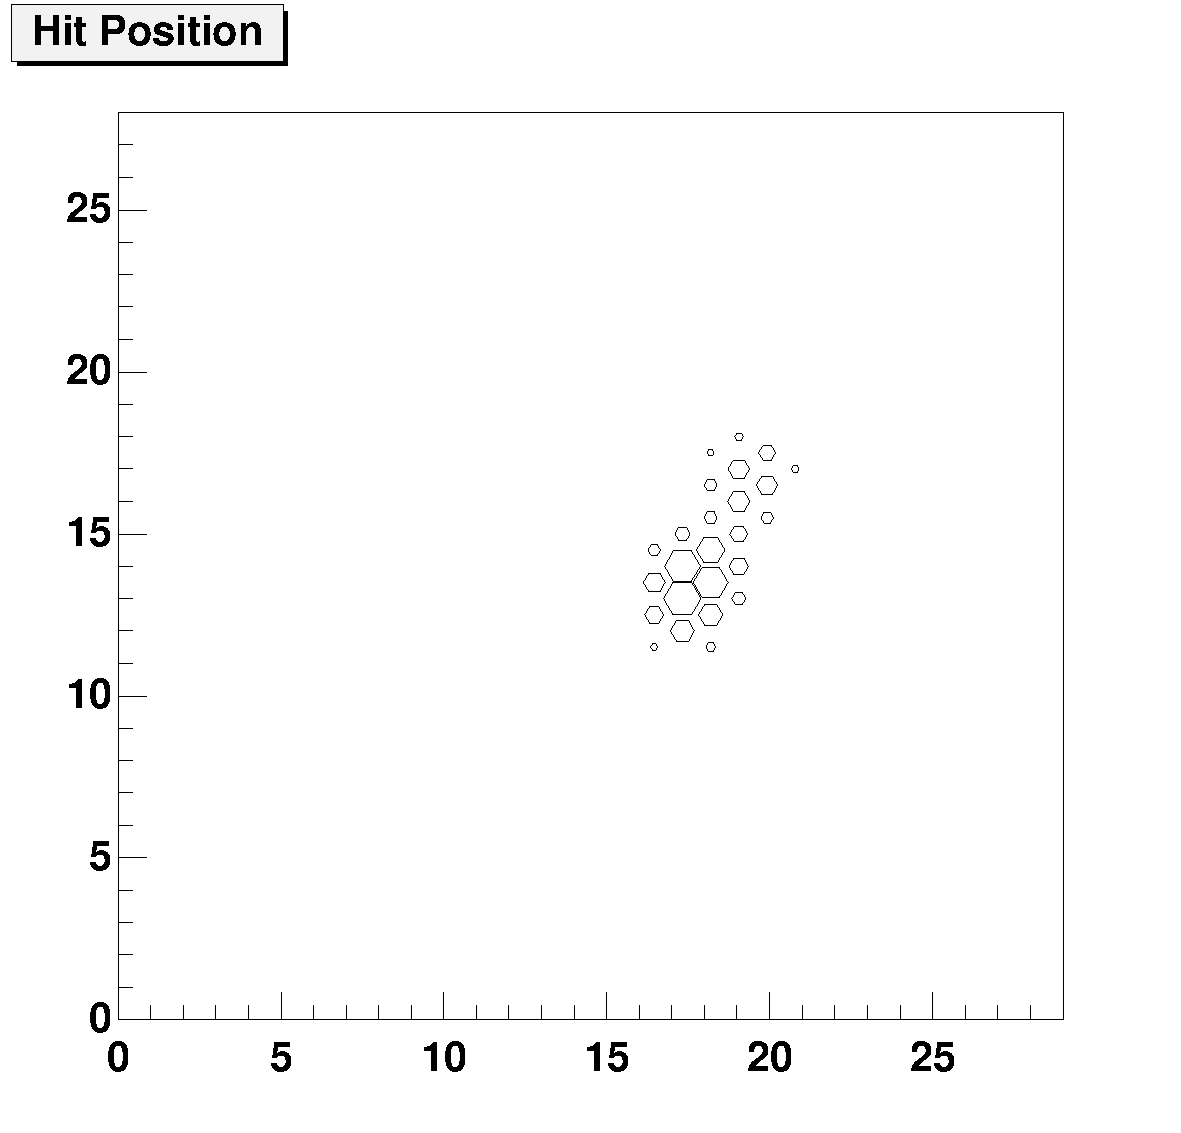
\includegraphics[width=5.8cm]{./ps_LaTeX/figure/test.pdf}
\end{center}
\caption{Questa \`e una figura di esempio.}
\label{figura_di_esempio}
\end{figure}
La prima cosa che dobbiamo fare \`e includere un pacchetto specifico, e
questo si fa inserendo all'interno del preambolo il comando:
\begin{verbatim}
\usepackage[dvips]{graphicx}
\end{verbatim}
Fatto questo, grafici ed immagini in formato eps%
\footnote{
Il formato eps (\emph{Encapsulated PostScript}) \`e piuttosto usato,
specialmente nella comunit\`a scientifica, per la creazioni di grafici,
schemi sintetici ed oggetti di grafica vettoriale in generale (sostanzialmente
tutto ci\`o che \`e costituito da linee, punti e lettere).
Vedremo nel prossimo capitolo come creare grafici eps utilizzando il programma
di analisi dati \gnuplot.
}
possono essere inseriti con poche linee (il risultato della compilazione
appare in figura~\ref{figura_di_esempio}):
\begin{verbatim}
\begin{figure}[!htb]
\begin{center}
\includegraphics[width=5.8cm]{./ps_LaTeX/figure/Test.eps}
\end{center}
\caption{Questa \`e una figura di esempio.}
\label{figura_di_esempio}
\end{figure}
\end{verbatim}

Sostanzialmente non vi \`e niente di nuovo se non l'ambiente (flottante)
\cchar{figure}, per cui vale quanto detto a proposito di \cchar{table},
ed il comando:
\begin{verbatim}
\includegraphics[width=8cm]{./ps_LaTeX/figure/Test.eps}
\end{verbatim}
cui \`e passato il nome del \emph{file} eps come argomento e la larghezza
con cui l'immagine in esso contenuta deve apparire nel documento.
Notiamo, per inciso, che ``\verb|\includegraphics|'' \`e il comando che
richiede il pacchetto \cchar{graphicx}.

Si possono ovviamente anche inserire figure in formato diverso dal
postscript (ad esempio jpg, png etc.). L'unica differenza \`e che in questo
caso bisogna specificare esplicitamente le dimensioni dell'immagine%
\footnote{
Tecnicamente questo \`e conseguenza del fatto che il formato eps, a differenza
degli altri, contiene al suo interno la definizione della cosiddetta
\emph{bounding box}.
}
tra le opzioni di ``\verb|\includegraphics|''.
Se, per esempio, supponiamo di voler inserire una figura in formato jpg
di $800\times 600$ pixel, dovremo scrivere qualcosa del tipo:
\begin{verbatim}
\includegraphics[width=8cm, bb=0 0 800 600]{./Figura.jpg}
\end{verbatim}
in cui il frammento \cchar{bb=0 0 800 600}
fornisce appunto la dimensione della \emph{cornice} che racchiude l'immagine
(cio\`e della \emph{bounding box}), nella forma delle coordinate (espresse in
pixel) degli angoli in alto a sinistra (\cchar{0 0}) ed in basso a destra
(\cchar{800 600}) della cornice stessa.
.
